\chapter{Exact intensity for the two-faceted cup}\label{app:boundariescup}
For very simple optical systems, the \textit{exact} target intensity of light can be calculated. Here we explain how this is done for the two-faceted cup formed by a Lambertian source described in Chapter \ref{chap:raytracing}. We remind the reader that, for this system, the intensity in a given direction $\variabile{p}$ in PS is defined as:
\begin{equation}\label{eq:eta_appendix}
I_{\textrm{PS}}(\variabile{p}) = \sum_{\Pi}\int_{\variabile{q}^\textrm{\,min}(\Pi, \variabile{p})}^{\variabile{q}^\textrm{\,max}(\Pi,\variabile{p})}L(\variabile{q}, \variabile{p})\textrm{d}\variabile{q} = \sum_{\Pi}\big (\variabile{q}^\textrm{max}(\Pi,\variabile{p})-\variabile{q}^\textrm{\,min}(\Pi,\variabile{p})\big )\,,
\end{equation}
where the sum is over all the possible paths, $\variabile{q}^\textrm{\,min}(\Pi,\variabile{p})$ and $\variabile{q}^\textrm{\,max}(\Pi,\variabile{p})$ are the minimum and maximum position coordinates of the rays on $\partial$\insieme{R}$_\textrm{t}(\Pi)$ along direction $\variabile{p}$, and the second equation holds as we assume $L=1$ in \insieme{R}$_\textrm{t}(\Pi)$.
Therefore, if we are able to provide an analytic expression for the boundaries $\partial$\insieme{R}$_\textrm{t}(\Pi)$ we can calculated the position coordinates $\variabile{q}^\textrm{\,min}(\Pi,\variabile{p})$ and $\variabile{q}^\textrm{\,max}(\Pi,\variabile{p})$ of the intersection points between the line $\variabile{p}=\textrm{const}$ and $\partial$\insieme{R}$_\textrm{t}(\Pi)$ analytically and the exact intensity for every direction $\variabile{p}$ is obtained using (\ref{eq:eta_appendix}). The procedure used for such purpose is explained next.
\section{Analytic approach}
The idea is to rotate the cup to determine the maximum number of reflections between the rays and the optical lines before reaching the target. The rays are considered to be straight lines instead of broken lines. Hence it is sufficient to find only one intersection point between the ray and a line segment (also in the case where more than one reflection occurs). Finally transforming back these points we obtain the corresponding coordinates at the target.\\ \indent
The two-faceted cup is defined in the $(\variabile{x}, \variabile{z})$-plane as in Chapter \ref{chap:raytracing}. 
Let $\gamma\in[0, \pi/2]$ be the angle that the left and right reflector make with the normal to the source. 
%\begin{figure}[t]
%\label{fig:cup}
%  \begin{center}
%%\vspace{-1.5cm}
%  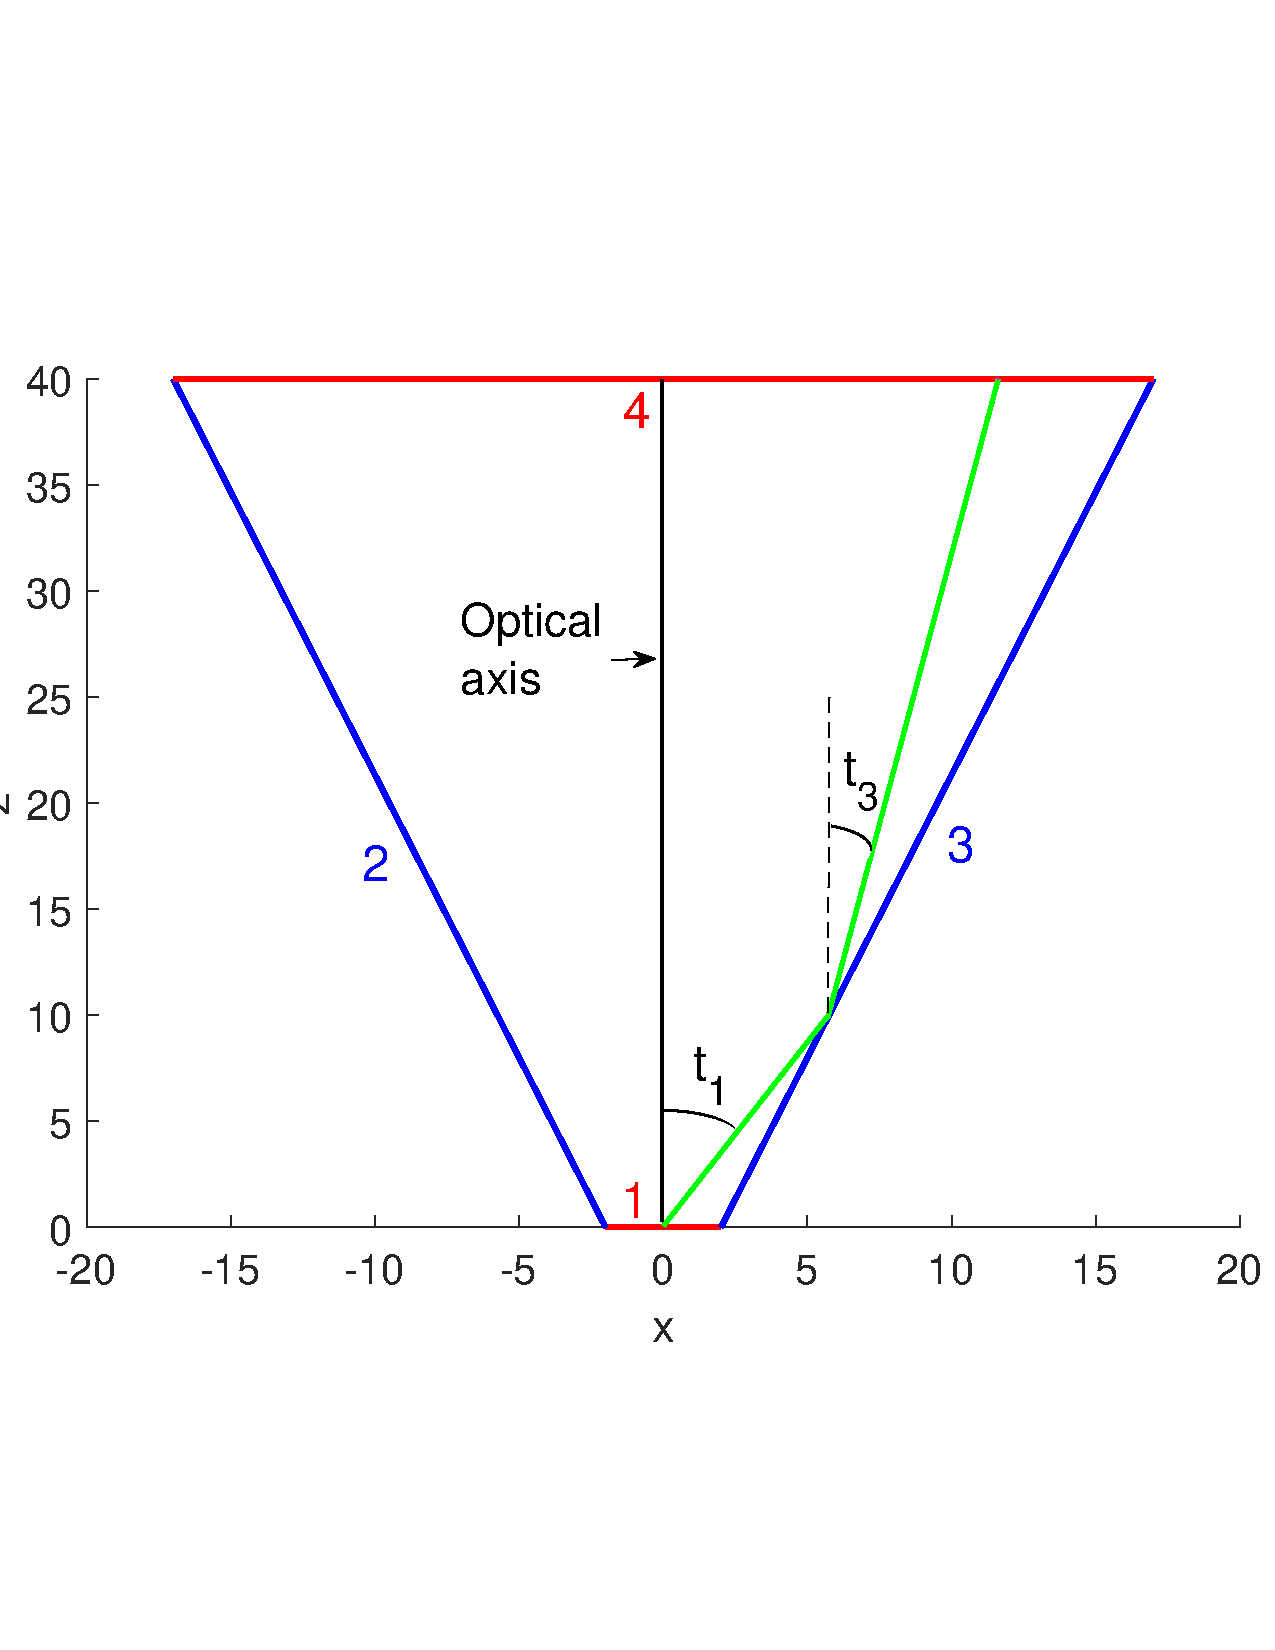
\includegraphics[width=6.7cm]{cup.pdf}
%  \end{center}
%%\vspace{-2cm}
%  \caption{\textbf{Shape of the two-faceted cup.}  Each line of the system is labeled with a number.
%   The source \point{S}$= [-2,2]$ (line number $1$) is located on the $\variabile{x}$-axis.
%   The target \point{T}$= [-17, 17]$ (line $4$) is parallel to the source and is located at a height $\variabile{z}= 40$.
%   The left and right reflectors (line $2$ and $3$) connect the source with the target.}
%  \label{fig:cup}
%\end{figure}
The maximum $\variabile{z}$-coordinate that the two-faceted cup can reach during the rotation is defined by:
\begin{equation}\label{rotation}\begin{tabular}{llll}
$Z$ & $=$ & $ \big(h+\frac{\variabile{a}}{\tan\gamma}\big)\frac{1}{\cos\gamma}-\frac{\variabile{a}}{\tan\gamma}$ \\ $ \quad$ & $ \quad $ & $ \quad $ \\$ \quad$ &  $=$ & $\frac{h}{\cos\gamma}+\frac{\variabile{a}(1-\cos\gamma)}{\sin\gamma}\big),$\end{tabular}
\end{equation} and $\point{R}=(0,-\frac{\variabile{a}}{\tan\gamma})$ is the rotation point. We define $\point{B}_k$ as the clockwise ($k<0$) or counterclockwise ($k\geq 0$) rotation image around the point $\point{R}$ over an angle $\alpha_k=(2k+1)\gamma$, with $k$ an integer number (Figure \ref{fig:twofaced} is illustrative).
\begin{figure}[t]%\label{fig:twofaced}
 \centering
  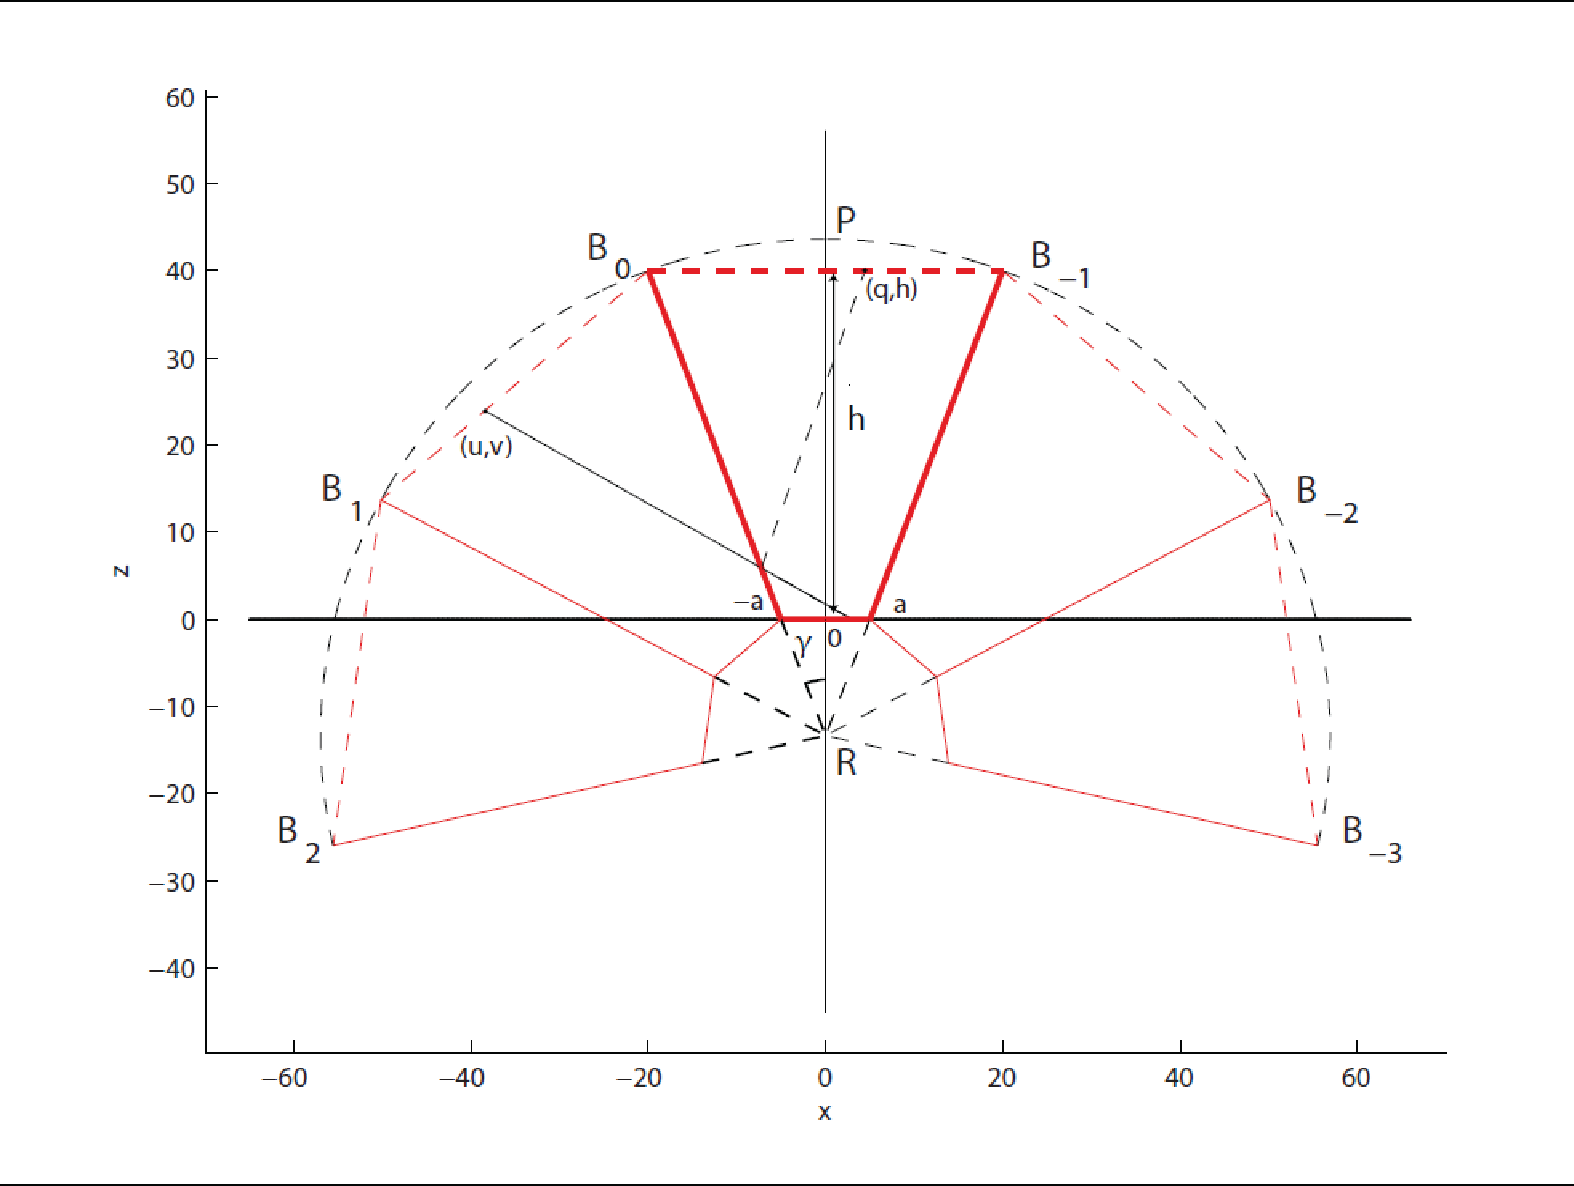
\includegraphics[width=\textwidth]{rotated_cup.pdf}
 \caption{\textbf{The two-faceted cup rotated twice on both sides.} The line segment with end points $B_{k-1}$ and $B_{k}$ is the $|k|$ times rotated target. The coordinates $(q,h)$ on the target $B_{-1}B_{0}$ are obtained by transforming the coordinates $(u,v)$ of the intersection point between a ray and the segment $B_0B_1$ . The point $\point{R} = \big(0,-\frac{a}{\tan{\gamma}}\big)$ is the center of the circle described by rotating the cup (dashed line).}
  \label{fig:twofaced}
  \end{figure}
  %as the notation used in equation ($\ref{Bk}$) could suggest.
The position coordinates of points $\point{B}_k = (B_{k,x}, B_{k,z})$ are given by:
\begin{equation}
 \begin{pmatrix} B_{k,x}  \\  B_{k,z}\end{pmatrix}= -
  \begin{pmatrix} 0  \\  \frac{a}{\tan\gamma}\end{pmatrix}+
 \left(\begin{split}  & \cos\alpha_k  & -\sin\alpha_k \\  & \sin\alpha_k & \cos\alpha_k\end{split}\right).
 \begin{pmatrix}  0 \\  Z+\frac{a}{\tan\gamma}\end{pmatrix},
\end{equation}
The maximum number of reflections $r_{\textrm{max}}$ a ray can undergo before arriving at the target is:
\begin{equation}
r_{\textrm{max}}=\max\{k\in\mathbb{N} \;| \; B_{k-1,z}\geq 0\}
\end{equation}
because rays cannot reach $\variabile{z}<0$.
For example, for the two-faceted cup depicted in Figure \ref{fig:cup}, we found $r_{\textrm{max}}=2$.\\ \indent 
Given the coordinates $(\variabile{x}_1, \variabile{z}_1)$ and the angular coordinate $\optangle_1$ of a ray at the source we can calculate the corresponding position $(\variabile{x}, \variabile{z})$ and direction coordinate $\optangle$ at the target as explained in the following. \\ \indent We compute the coordinates $(u,v)$ of the intersection point between the ray parametrization and the $|\variabile{k}|$ times rotated or reflected target $\point{B}_{\variabile{k}-1}\point{B}_\variabile{k}$ for which the intersection with the forward ray is not empty where $\variabile{k}=-\variabile{r}_{\textrm{max}}-1, \cdots, \variabile{r}_{\textrm{max}}$. Next, if $\variabile{k}$ is even, the corresponding coordinates $(\variabile{x},\variabile{z})$ at the target are found by rotating back the coordinates $(\variabile{u},\variabile{v})$, otherwise a reflection is applied. Therefore, the ray coordinates $(\variabile{x},\variabile{z})$ at the target are given by:
\begin{equation} \label{rotation_target}\begin{pmatrix} \variabile{x}\\ \variabile{z}
\end{pmatrix} = \left(\begin{array}{cc}(-1)^k & 0  \\ 0 & 1\end{array}\right)
\left(\begin{array}{cc}\cos(-2\variabile{k}\gamma) & -\sin(-2\variabile{k}\gamma) \\\sin(-2\variabile{k}\gamma) & \cos(-2\variabile{k}\gamma)\end{array}\right)\begin{pmatrix} \variabile{u} \\
 \variabile{v}+\frac{a}{\tan(\gamma)}\end{pmatrix}-\begin{pmatrix}0 \\ \frac{a}{\tan\gamma}\end{pmatrix}.
\end{equation} We observe that the sign depends on the parity of $\variabile{k}$. When $\variabile{k}=0$, i.e., the ray does not reflect, the first two matrices become the identity matrix and the cup is not rotated nor reflected. When $\variabile{k}$ is even, the determinant of the matrix given by the product between the first and the second matrix (\ref{rotation_target}) is equal to $1$ and we obtained a rotation matrix, while when $\variabile{k}$ is odd the determinant of the product matrix is $-1$ and we have a reflection matrix.
\\ \indent
The method of transforming the cup instead of the rays allows us to determine the positive luminance regions $\mbox{\insieme{R}}_1(\Pi_{\variabile{j}})$ and $\mbox{\insieme{R}}(\Pi_{\variabile{j}})$ in source and target PS, where every path $(\Pi_{\variabile{j}})_{\variabile{j}=1, \cdots, 2\variabile{r}_{\textrm{max}}+1}$ corresponds to $|\variabile{k}|$ of reflections. The corresponding boundaries only consist of rays that either leave the extremes of the source or hit one of the points $\point{B}_\variabile{k}$. 
%At the boundaries a small change in the position or direction ray coordinate can cause a difference in the number of the reflections. 


Rays that leave the interior of \point{S} and hit $\point{B}_\variabile{k}$ have as position coordinates in source PS $\variabile{q}_1 = \variabile{x}_1\in(-\variabile{a}, \variabile{a})$, the corresponding target PS coordinates are $\variabile{q} = \variabile{x} = B_{\variabile{k}, \variabile{x}}$.
The direction coordinates of these rays at the source PS are $\variabile{p}_1 = \sin(\optangle_1)$ where $\optangle_1$ is given by:
\begin{equation}\label{anglesource}
\optangle_1 = \arctan\bigg(\frac{\variabile{x}_1-B_{k,x}}{B_{k,z}}\bigg).
\end{equation}
The corresponding direction coordinates at the target PS are $\variabile{p}=\sin(\optangle)$ where $\optangle$ is given by:
\begin{equation}\label{teta}
\optangle=(-1)^\variabile{k}(\optangle_1-2\variabile{k}\gamma).
\end{equation}

Rays emitted from the end points of the source have a constant position coordinate $\variabile{q}_1 = \variabile{x}_1 = \textrm{const}$ in source PS while varying the direction coordinate $\variabile{p}_1 = \sin(\optangle_1)\in[-1, 1]$ where $\optangle_1\in[-\pi/2, \pi/2]$. The corresponding target position coordinates $\variabile{x}$ is obtained from (\ref{rotation_target}) while the direction coordinates in the target PS are $\variabile{p} = \sin(\optangle)$, where $\optangle$ is given by Equation (\ref{teta}) and $\optangle_1\in[-\pi/2, \pi/2]$.
Note that the rays emitted from the end points of the source form vertical lines in source PS as $\variabile{q}_1= \textrm{const}$ while varying $\variabile{p}_1\in[-1,1]$.
On the other hand, rays that hit points $\point{B}_k$ form vertical lines in target PS as $\variabile{q} = \textrm{const}$ while varying $\variabile{p}\in[-1,1]$.
\\ \indent 
%In Figure \ref{fig:raggi} are shown some rays that compose the boundaries of $M_{\textrm{s},k}$ which coordinates are:
%$$ \begin{array}{cc}ADE = \Bigg(-a, \arctan\Big(\frac{-a+b_{-1,x}}{b_{-1,z}}\Big)\Bigg),\; ACE = \big(-a, \sin(\gamma)\big),\; AF = \big(-a, -\sin(\delta)\big), \\
% BCF = \Bigg(a, \arctan\Big(\frac{a-b_{1,x}}{b_{1,z}}\Big)\Bigg), BDF = \big(a, - \sin(\gamma)\big) \, \;\mbox{and} \,\; BE = \big(a, \sin(\delta)\big).\end{array} $$
%\begin{figure}
%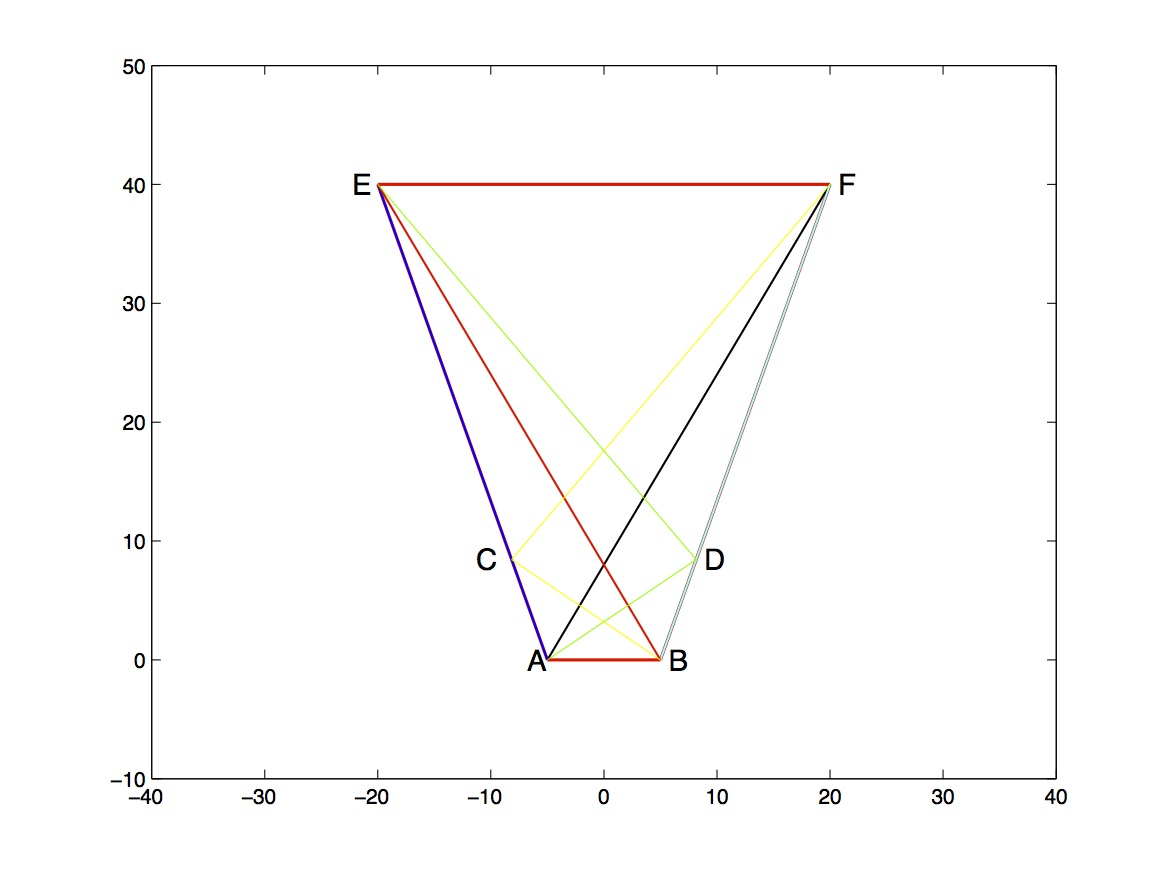
\includegraphics[scale=0.55]{raggi6.jpg}
%\caption{\footnotesize{Rays that leave the corner points of the source. The rays $AF$, $BE$, $ACE$, $BDF$ are rays that do not hit the reflectors of the system.
%They constitute rays on the boundaries of the regions $M_{\textrm{s},0}$, $M_{\textrm{s},1}$ and $M_{\textrm{s},-1}$.
% The rays $ADE$ and $BCF$ are rays that hit once the reflectors of the system. They constitute rays on the boundaries of the regions
% $M_{\textrm{s},-1}$, $M_{\textrm{s},-2}$, and $M_{\textrm{s},1}$ or $M_{\textrm{s},2}$, respectively.}}
%\label{fig:raggi}
%
%\end{figure}
%$$ \begin{array}{cc}ADE = \big(-b, -(t_1+2\gamma)\big)),\; ACE = \big(-b, \sin(\gamma)\big),\; AF = \big(-b, -\sin(\delta)\big), \\
% BCF = \big(b, -(t_2-2\gamma)\big), BDF = \big(b, - \sin(\gamma)\big) \, \;\mbox{and} \,\; BE = \big(b, \sin(\delta)\big).\end{array} $$
% where $t_1 = \arctan(\frac(-a+b_{-1,x}{b_{-1}}))$ and $t_2 = \arctan(\frac(a-b_{-1,x}{b_{-1}}))$.
The boundaries at the source and target PS are shown in red in Figures \ref{fig:boundary} and \ref{boundaries_target}, respectively. 
\begin{figure}[htbp]
\centering
%\begin{minipage}[t]{.40\textwidth}
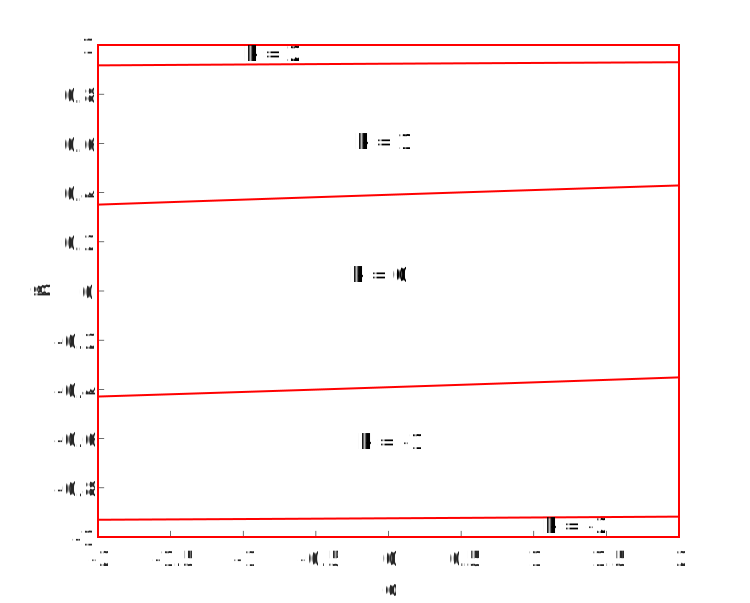
\includegraphics[width = 0.8 \textwidth]{analytic_boundaries_source}
\caption{Regions in source PS formed by rays that reflect $|k|$ times, for the two-faceted cup in Figure \ref{fig:cup}.}
\label{fig:boundary}
%\end{minipage} \qquad \qquad
%\begin{minipage}[t]{.40\textwidth}
\end{figure}
\begin{figure}[htbp]
\centering
%\begin{minipage}[t]{.40\textwidth}
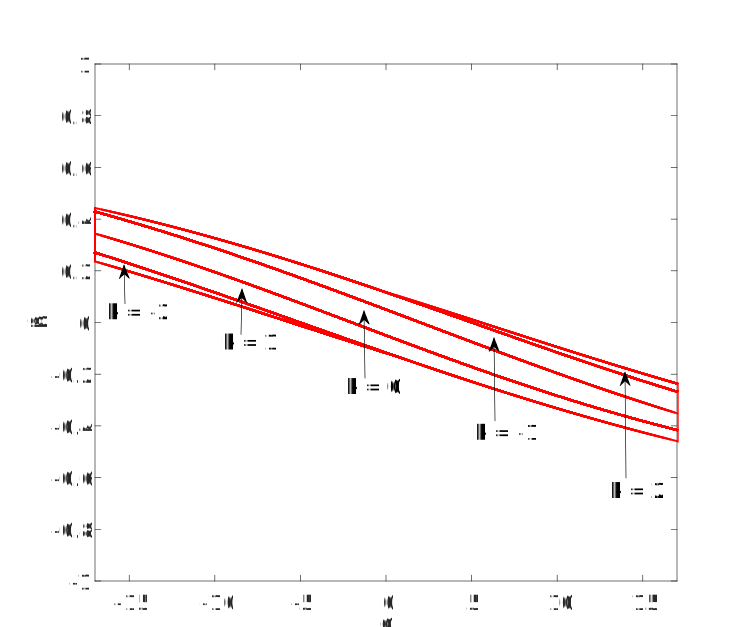
\includegraphics[width = 0.8 \textwidth]{analytic_boundaries_target}
\caption{Regions in target PS formed by rays that reflect $|k|$ times, for the two-faceted cup in Figure \ref{fig:cup}.}
\label{boundaries_target}
%\end{minipage} \qquad \qquad \qquad
\end{figure}
%\noindent 
%Figure \ref{fig:boundary} and \ref{boundaries_target} show also the symmetry of the regions $M_{\textrm{s},k}$ and $M_{\textrm{t},k}$. 
%Finally we note that, since $k = 1$ is odd, the position of the regions $M_{\textrm{t},1}$ and $ M_{\textrm{t},-1}$ are exchanged with respect to the position of $ M_{\textrm{s},1}$ and $ M_{\textrm{s},-1}$.
Once the boundaries at the target are determined, the coordinates of the intersection points between line $\variabile{p}=\textrm{const}$ and $\partial$\insieme{R}$(\Pi_{\variabile{j}})$ are found for every path $(\Pi_\variabile{j})_{\variabile{j}=1, \cdots, 2\variabile{k}+1}$ along every direction $\variabile{p}$. The target intensity is computed using Equation (\ref{eq:eta_appendix}). The intensity profile is depicted in Figure \ref{fig:intensity_cup_analytic}. 
\begin{figure}[htbp]
\centering
%\begin{minipage}[t]{.40\textwidth}
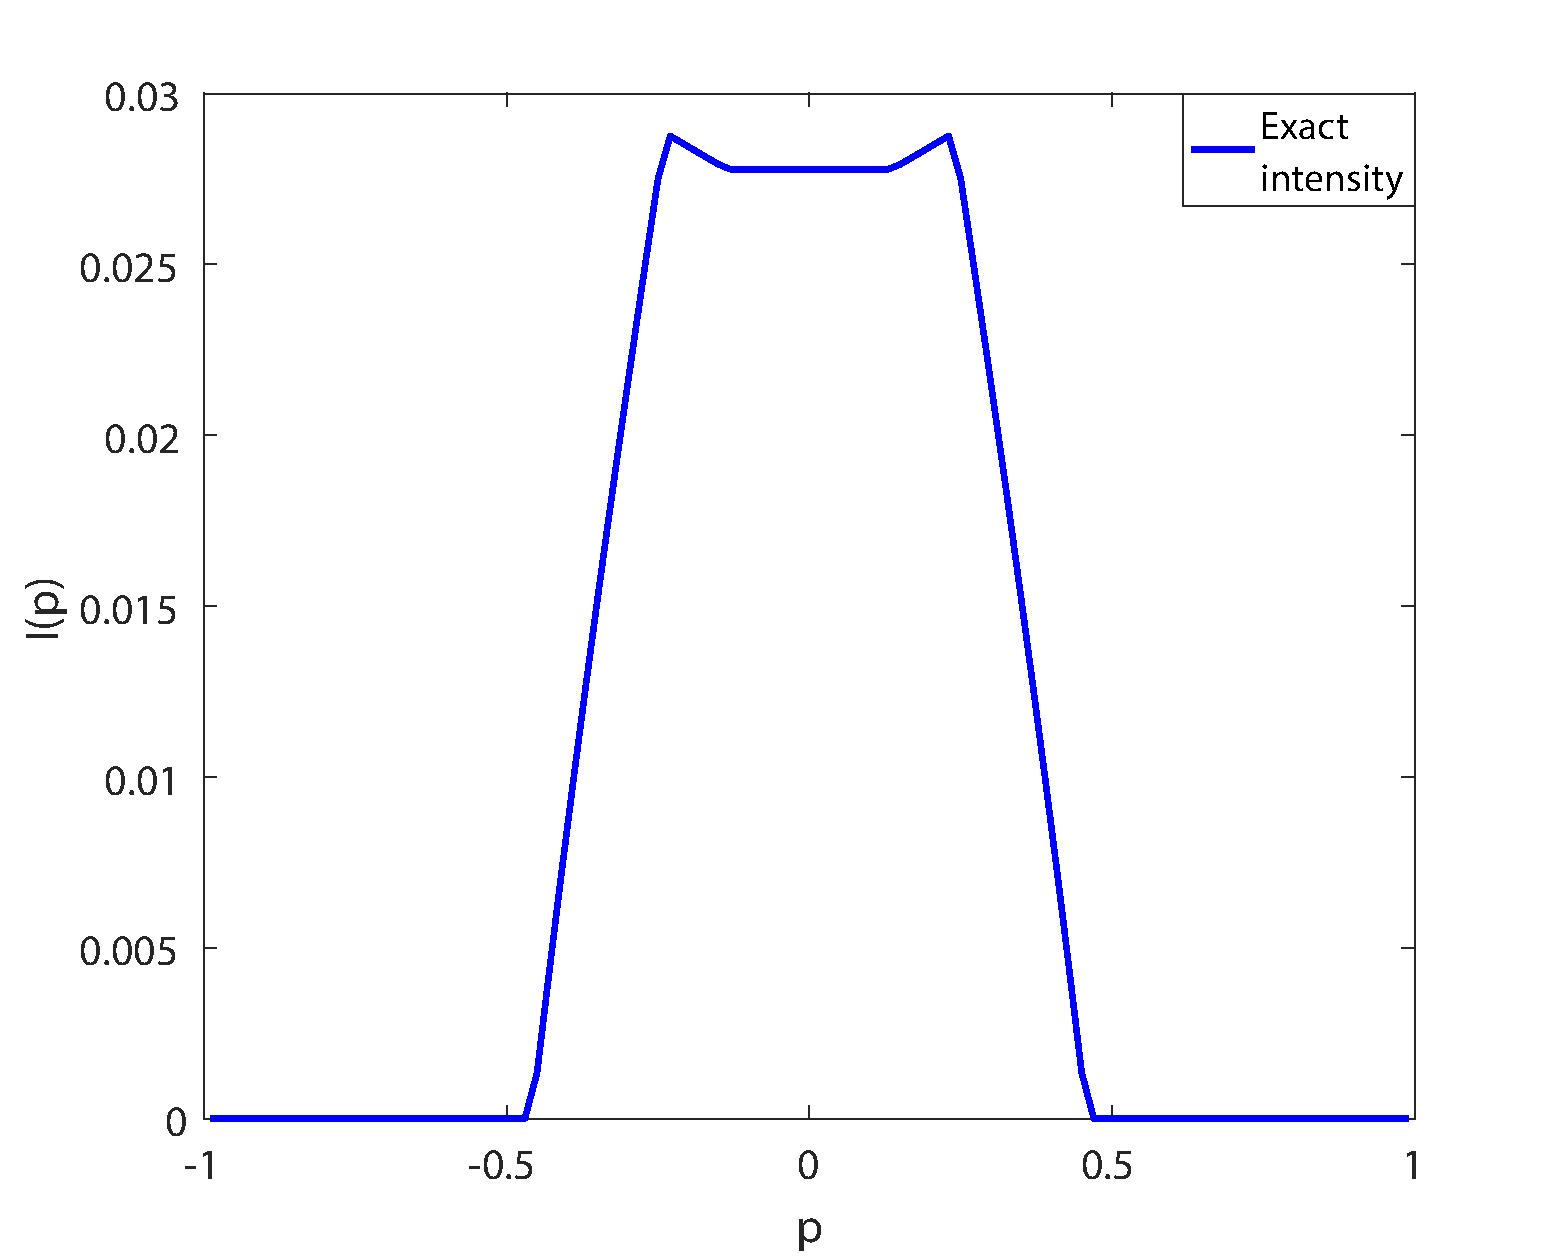
\includegraphics[width = 0.7\textwidth]{Exact_intensity}
\caption{Profile of the exact intensity at the target of the two-faceted cup.}
\label{fig:intensity_cup_analytic}
%\end{minipage} \qquad \qquad \qquad
\end{figure}
Since the boundaries are calculated analytically, the intensity $I(\variabile{p})$ found is the exact intensity.

The exact intensity found as described above was taken as reference intensity in Chapters \ref{chap:triangulation} and \ref{chap:raymapping1}.

